\documentclass{standalone}
\usepackage{tikz}
\begin{document}
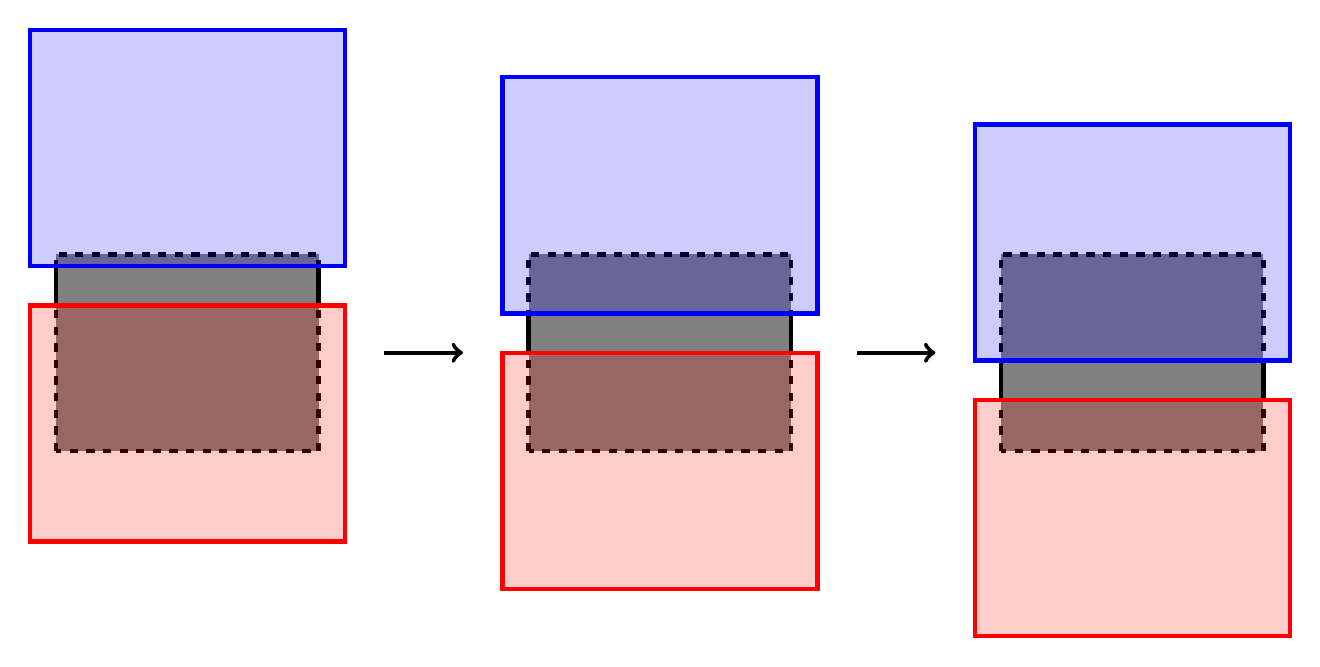
\begin{tikzpicture}

\def\sceneW{6cm}
\def\sceneWW{4.5cm}
\def\sceneSpace{1cm}
\def\planeW{4}
\def\planeH{3}
\def\planeSep{-0.1}
\def\backW{3.333}
\def\backH{2.5}
\def\backX{0.333}
\def\backY{0.25}
\def\clrfirst{red}
\def\clrsecond{blue}
\def\clrback{black}
\def\slitsize{0.5}

\newcommand{\render}[1]{%
	% shutter
	\draw [\clrback,fill=gray,dashed] (\backX,\backY) rectangle ++(\backW, \backH);
	\draw [\clrback,fill=gray] (\backX,\planeH+\planeSep-#1)
	-- ++(0,-\slitsize) ++(\backW,0) -- ++(0,\slitsize);
	% top
	\draw [\clrsecond,fill,fill opacity=0.2] (0,\planeH+\planeSep-#1) rectangle ++(\planeW, \planeH);
	% bottom
	\draw [\clrfirst,fill,fill opacity=0.2] (0,\planeSep-#1-\slitsize) rectangle ++(\planeW,\planeH);
}
\begin{scope}[ultra thick]
		\render{0.3}

		% scene move
		\draw [->] (\sceneWW,0.5*\planeH) -- ++(\sceneSpace,0);

	\begin{scope}[xshift = \sceneW]
		\render{0.9}

		% scene move
		\draw [->] (\sceneWW,0.5*\planeH) -- ++(\sceneSpace,0);
	\end{scope}

	\begin{scope}[xshift=2*\sceneW]
		\render{1.5}
	\end{scope}

\end{scope}

\end{tikzpicture}
\end{document}
